\documentclass{article}
\usepackage{fancyhdr}
\usepackage{lipsum}  
\usepackage{listings} 
\usepackage{xcolor}   
\usepackage{amsmath}
\usepackage{enumitem}
\usepackage{graphicx}
\usepackage{caption}
\usepackage{verbatim}

% Define macros for title and author
\newcommand{\thetitle}{STAT 641 \\ Homework 6}
\newcommand{\theauthor}{Keegan Smith}

\title{\thetitle}
\author{\theauthor}

\pagestyle{fancy}
\fancyhf{}  % Clear all header and footer fields
\fancyhead[L]{\nouppercase{\rightmark}}
\fancyhead[C]{\thetitle}  % Title in the center
\fancyhead[R]{\theauthor}  % Your name on the right

\lstset{ %
  backgroundcolor=\color{lightgray},   % choose the background color
  basicstyle=\ttfamily\small,          % size of fonts used for the code
  keywordstyle=\color{blue},           % color for keywords
  commentstyle=\color{green},          % color for comments
  stringstyle=\color{red},             % color for strings
  numbers=left,                        % where to put the line-numbers
  numberstyle=\tiny\color{gray},       % style for line-numbers
  stepnumber=1,                        % the step between two line-numbers
  numbersep=5pt,                       % how far the line-numbers are from the code
  frame=single,                        % adds a frame around the code
  rulecolor=\color{black},             % frame color
  breaklines=true,                     % automatic line breaking
  breakatwhitespace=false,             % automatic breaks should only happen at whitespace
  showspaces=false,                    % don't show spaces in the code
  showstringspaces=false,              % don't show spaces in strings
  showtabs=false,                      % don't show tabs in the code
}

\begin{document}

\maketitle
\section*{Problem 1}
\begin{enumerate}
\item To create a reference plot, we must first make it such that the Weibull is a location-scale distribution. We can accomplish this (as outlined in Handout 8) by applying the transformation: \\
\[
X = \log(Y)
\]
so if $X$ follows a log-Weibull distribution, then $Y$ follows a Weibull distribution. \\
The cdf of the log weibull is: \\
\begin{align*}
P(\ln(Y) \leq x) &= P(Y \leq e^x) \\
&= 1 - e^{-(\frac{e^x}{\alpha})^\gamma} \\
&= 1 - e^{-e^{\frac{x - \theta_1}{\theta_2}}}
\end{align*}
We can then solve for the quantile function: \\
\begin{align*}
s &= 1 - e^{-e^{\frac{x - \theta_1}{\theta_2}}} \\
\ln(-s + 1) &= -e^{\frac{x - \theta_1}{\theta_2}} \\
\ln(-\ln(-s + 1)) &= \frac{x - \theta_1}{\theta_2} \\
\theta_2 \cdot \ln(-\ln(-s + 1)) + \theta_1 &= x \\
\end{align*}
Thus we have: \\
\[
Q_z(u) = \ln(-\ln(-u + 1))
\]
We can then make the reference plot with the following R code (continued from the previous R code):
\begin{verbatim}\
x <- c(0.8402, 1.0644, 1.1298, 1.4314, 1.7795, 1.9121, 2.2343, 2.3424, 2.3559, 2.3855,
2.5734, 2.5815, 2.5893, 2.7562, 2.9040, 2.9295, 3.1124, 3.5490, 3.7684, 3.7953,
3.8846, 3.9766, 4.1918, 4.3887, 4.7106, 4.8918, 4.9716, 6.5018, 7.0740, 7.2158)
y = -log(x)
y = sort(y)
n = length(y)
weib= -y
weib= sort(weib)
i= 1:n
ui= (i-.5)/n
QW= log(-log(1-ui))
plot(QW,weib,abline(lm(weib~QW)),
main="Weibull Reference Plot",cex=.75,lab=c(7,11,7),
xlab="Q=ln(-ln(1-ui))",
ylab="y=ln(W(i))")
\end{verbatim}
\begin{figure}[htbp]
    \centering
    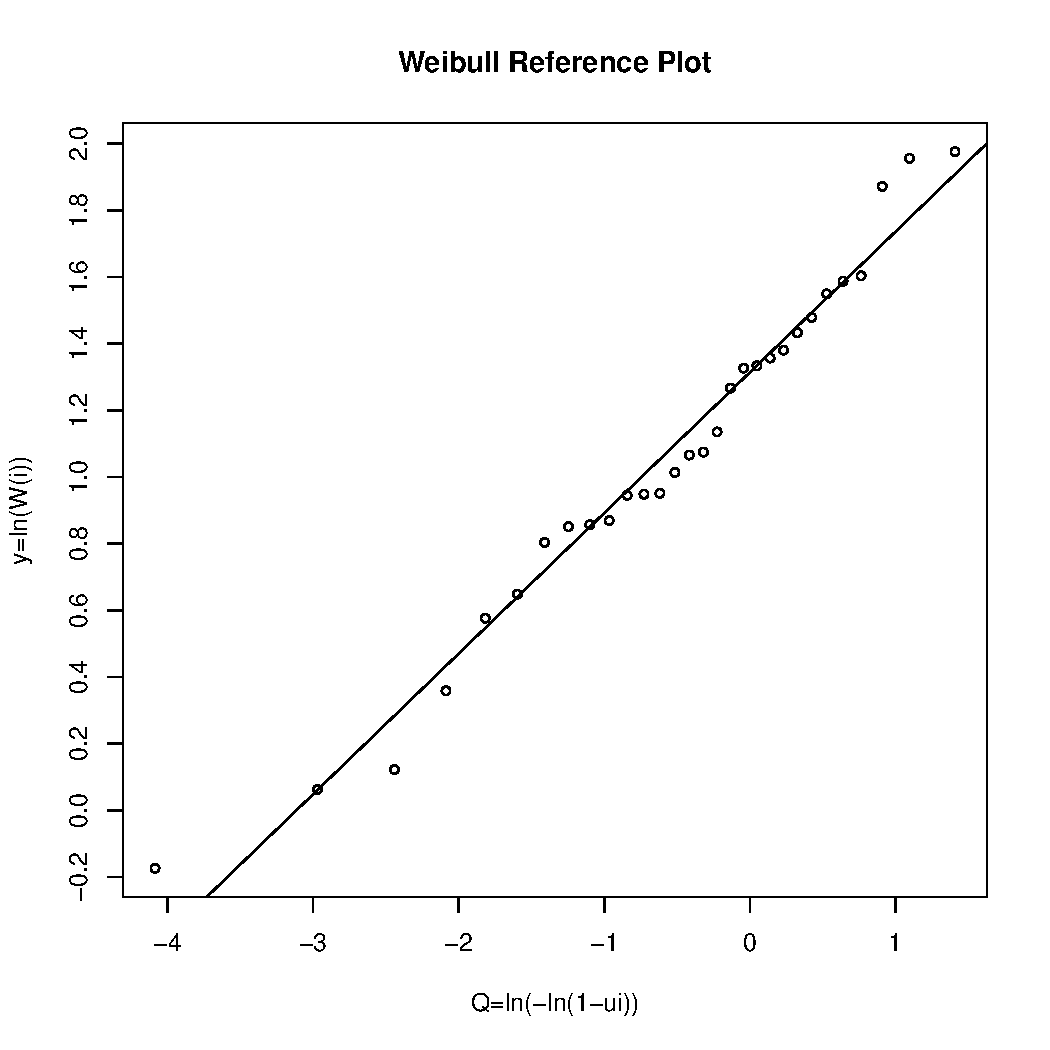
\includegraphics[width=0.8\textwidth]{Rplots.pdf}
\end{figure}
\newpage
We will also compute the Anderson-Darling GOF test in R: \\
\begin{verbatim}
library(MASS)
mle <- fitdistr(x,"weibull")
shape = mle$estimate[1]
scale = mle$estimate[2]
a = -log(scale)
b = 1/shape
z = exp(-exp(-(y-a)/b))
A1i = (2*i-1)*log(z)
A2i = (2*n+1-2*i)*log(1-z)
s1 = sum(A1i)
s2 = sum(A2i)
AD = -n-(1/n)*(s1+s2)
ADM = AD*(1+.2/sqrt(n))
AD
ADM
\end{verbatim}
This results in $A^2 = 0.3059062$. From the table in Handout 9, this corresponds with a p-value $> .25$. Combining this with the fact that the reference plot is fairly straight, I am inclined to say the Weibull distribution is a good fit for the data.
\item We can solve for the CI for the upper quantile using the following R code (adapted from handout 11): \\
\begin{verbatim}
x <- c(0.8402, 1.0644, 1.1298, 1.4314, 1.7795, 1.9121, 2.2343, 2.3424, 2.3559, 2.3855,
2.5734, 2.5815, 2.5893, 2.7562, 2.9040, 2.9295, 3.1124, 3.5490, 3.7684, 3.7953,
3.8846, 3.9766, 4.1918, 4.3887, 4.7106, 4.8918, 4.9716, 6.5018, 7.0740, 7.2158)
n=length(x)
L=.95
P=.75
s=ceiling(n*P)-1
r=floor(n*P)+1
cov=0
while(s<n-1 && r>1 && cov<L)
{s=s+1
cov=pbinom(s-1,n,P)-pbinom(r-1,n,P)
if(cov>=L) break;
r=r-1
cov=pbinom(s-1,n,P)-pbinom(r-1,n,P)
}
x[r]
x[s]
cov
\end{verbatim}
this results in the 95\% confidence interval $[3.549, 6.5018]$ with coverage probability .9678
\item We will assume the survival times of engines are independent. We will use power transformations (as outlined in handout 9) to transform the data to a somewhat normal distribution. We can find the power $\theta$ to be used with the following code: \\
\begin{verbatim}
y <- c(0.8402, 1.0644, 1.1298, 1.4314, 1.7795, 1.9121, 2.2343, 2.3424, 2.3559, 2.3855,
2.5734, 2.5815, 2.5893, 2.7562, 2.9040, 2.9295, 3.1124, 3.5490, 3.7684, 3.7953,
3.8846, 3.9766, 4.1918, 4.3887, 4.7106, 4.8918, 4.9716, 6.5018, 7.0740, 7.2158)
n = length(y)
yt0 = log(y)
s = sum(yt0)
varyt0 = var(yt0)
Lt0 = -1*s - .5*n*(log(2*pi*varyt0)+1)
th = 0
Lt = 0
t = -3.01
i = 0
while(t < 3)
{t = t+.001
i = i+1
th[i] = t
yt = (y^t -1)/t
varyt = var(yt)
Lt[i] = (t-1)*s - .5*n*(log(2*pi*varyt)+1)
if(abs(th[i])<1.0e-10)Lt[i]<-Lt0
if(abs(th[i])<1.0e-10)th[i]<-0
}
# The following outputs the values of the likelihood and theta and yields
# the value of theta where likelihood is a maximum
out = cbind(th,Lt)
Ltmax= max(Lt)
Ltmax
imax= which(Lt==max(Lt))
thmax= th[imax]
thmax
\end{verbatim}
This yields $\theta = 0.325$. Thus the transformation is: \\
\[
Y = \frac{y^{.325} - 1}{.325}
\]
We can apply this transformation and find the 95\% CI of the mean of the new distribution with R: \\
\begin{verbatim}
y = (y^.325 - 1) / .325
mean = mean(y)
std = sd(y)
error = qnorm(0.975)*std/sqrt(n)
lower = mean - error
upper = mean + error
lower
upper
\end{verbatim}
we can then apply the inverse of the transformation function to get back the lower and upper bounds for the original distribution: \\
\begin{verbatim}
lower_transform = (lower * .325 + 1)^(1 / .325)
upper_transform = (upper * .325 + 1)^(1 / .325)
lower_transform
upper_transform
\end{verbatim}
This results in the 95\% CI of $[2.526999, 3.663964]$
\item For this, we will construct a two sided tolerance interval. First we will use a power transformation to normalize the data, then we will use the code from handout 11 for creating a two sided tolerance interval, and then we will back transform the interval endpoints: \\
\begin{verbatim}
y <- c(0.8402, 1.0644, 1.1298, 1.4314, 1.7795, 1.9121, 2.2343, 2.3424, 2.3559, 2.3855,
2.5734, 2.5815, 2.5893, 2.7562, 2.9040, 2.9295, 3.1124, 3.5490, 3.7684, 3.7953,
3.8846, 3.9766, 4.1918, 4.3887, 4.7106, 4.8918, 4.9716, 6.5018, 7.0740, 7.2158)
n = length(y)
yt0 = log(y)
s = sum(yt0)
varyt0 = var(yt0)
Lt0 = -1*s - .5*n*(log(2*pi*varyt0)+1)
th = 0
Lt = 0
t = -3.01
i = 0
while(t < 3)
{t = t+.001
i = i+1
th[i] = t
yt = (y^t -1)/t
varyt = var(yt)
Lt[i] = (t-1)*s - .5*n*(log(2*pi*varyt)+1)
if(abs(th[i])<1.0e-10)Lt[i]<-Lt0
if(abs(th[i])<1.0e-10)th[i]<-0
}
# The following outputs the values of the likelihood and theta and yields
# the value of theta where likelihood is a maximum
out = cbind(th,Lt)
Ltmax= max(Lt)
Ltmax
imax= which(Lt==max(Lt))
thmax= th[imax]
thmax

y = (y^thmax - 1) / thmax
G = .95
P = .95
Chi = qchisq(1-(1 - G) / 2,n-1)
z = qnorm((1+P)/2)
K2Side = sqrt(((n-1)*(n+1)*z^2)/(n*Chi))
lower = mean(y) - K2Side * sd(y)
upper = mean(y) + K2Side * sd(y)
lower_transform = (lower * thmax + 1)^(1 / thmax)
upper_transform = (upper * thmax + 1)^(1 / thmax)
lower_transform
upper_transform
\end{verbatim}
The result is that we can be 95\% confident that at least 95\% of values will fall in the interval [1.174811, 6.343665]
\end{enumerate}
\section*{Problem 2}
\begin{enumerate}

\item 
\begin{enumerate}
\item Adapting the code from handout 11: \\
\begin{verbatim}
y <- c(1.1, 2.6, 3.0, 3.7, 4.1, 6.5, 8.1, 9.1, 9.2, 11.7, 13.8, 14.3, 17.8, 19.3, 19.7,
22.7, 22.9, 23.4, 23.9, 24.9, 26.9, 27.4, 27.5, 28.7, 31.4, 35.9, 41.7, 42.5, 43.1,
45.4, 46.2, 48.3, 54.2, 54.4, 54.8, 60.7, 61.0, 70.0, 70.1, 70.2, 75.4, 75.4, 75.7,
76.6, 76.9, 76.9, 78.7, 80.6, 83.6, 85.7, 86.0, 87.4, 90.0, 93.4,94.3, 96.7, 96.8,
100.1, 105.4, 105.9, 110.9, 112.8, 113.3, 114.3, 114.9, 119.4, 119.5, 120.6, 121.0,
127.7, 129.5, 129.8, 133.3, 133.6, 136.0, 137.5, 137.6, 138.5, 140.1, 158.4, 158.7,
165.9, 166.0, 166.9, 169.2, 174.4, 183.7, 188.0, 227.9, 248.0, 257.6, 271.4, 280.9,
283.5, 287.8, 303.2, 308.1, 326.5, 334.9, 520.4)
n= length(y)
thest = mean(y)
B = 9999
thestS = numeric(B)
thestS = rep(0,times =B)
for (i in 1:B)
thestS[i] = mean(sample(y,replace=T))
RS= sort(thestS-thest)
LRS = RS[250]
URS = RS[9750]
thL = thest-URS
thU = thest-LRS
thL
thU
\end{verbatim}
This yields the interval $[86.876, 121.981]$
\item Again adapting the code from handout 11:
\begin{verbatim}
n= length(y)
thest = mean(y)
V = thest**2/n
B = 9999
W = numeric(B)
W = rep(0,times =B)
for (i in 1:B)
W[i] = mean(sample(y,replace=T))
Z = sqrt(n)*(W-thest)/W
Z = sort(Z)
LZ = Z[250]
UZ = Z[9750]
thL = thest-UZ*sqrt(V)
thU = thest-LZ*sqrt(V)
thL
thU
\end{verbatim}
Which results in the interval $[89.64146, 125.3428]$\\
\item We again adapt the code from handout 11: \\
\begin{verbatim}
n= length(y)
thest = mean(y)
V = thest**2/n
B = 9999
#calculate mle for lambda
lambda_hat <- 1 / thest 
for(i in seq_len(B)) {
  W[i] <- mean(rexp(n, rate = lambda_hat))
}
Z = sqrt(n)*(W-thest)/W
Z = sort(Z)
LZ = Z[250]
UZ = Z[9750]
thL <- thest - UZ * sqrt(V)
thU <- thest - LZ * sqrt(V)
thL
thU
\end{verbatim}
This results in the interval $[86.94429, 129.0083]$
\end{enumerate}
\item For basic bootstrap we have: \\
\begin{verbatim}
n = 100
B_sim = 50
true_mu = 100
count = 0
width_total = 0
for (i in 1:B_sim) {
  x_sim <- rexp(n, rate = 1/true_mu)
  thest = mean(x_sim)
  B = 9999
  thestS = numeric(B)
  thestS = rep(0,times =B)
  for (i in 1:B)
  thestS[i] = mean(sample(x_sim,replace=T))
  RS= sort(thestS-thest)
  LRS = RS[249] #handout was wrong, wasn't doing 0 indexing.... too lazy to fix it in my previous work. 
  URS = RS[9749]
  thL = thest-URS
  thU = thest-LRS
  width = thU - thL
  width_total += width
  if (thL <= true_mu && true_mu <= thU) {
    count <- count + 1
  }
}

cov <- count / B_sim
cov
width_avg = width_total / B_sim
width_avg
\end{verbatim}
which yields coverage $.96$ and average width 38.66296. \\
For studentized we have: \\
\begin{verbatim}
n = 100
B_sim = 50
true_mu = 100
count = 0
width_total = 0
for (i in 1:B_sim) {
    x_sim <- rexp(n, rate = 1/true_mu)
    thest = mean(x_sim)
    V = thest**2/n
    B = 9999
    W = numeric(B)
    W = rep(0,times =B)
    for (i in 1:B)
    W[i] = mean(sample(x_sim,replace=T))
    Z = sqrt(n)*(W-thest)/W
    Z = sort(Z)
    LZ = Z[250]
    UZ = Z[9750]
    thL = thest-UZ*sqrt(V)
    thU = thest-LZ*sqrt(V)
    width = thU - thL
    width_total = width_total + width
    if (thL <= true_mu && true_mu <= thU) {
        count <- count + 1
    }
}

cov <- count / B_sim
cov
width_avg = width_total / B_sim
width_avg
\end{verbatim}
Which yields a coverage of .98 and an average width of 39.16417 \\
For parametric bootstrap we have: \\
\begin{verbatim}
n = 100
B_sim = 50
true_mu = 100
count = 0
width_total = 0
for (i in 1:B_sim) {
    x_sim <- rexp(n, rate = 1/true_mu)
    thest = mean(x_sim)
    V = thest**2/n
    B = 9999
    W = numeric(B)
    W = rep(0,times =B)
    lambda_hat <- 1 / thest 
    for(i in seq_len(B)) {
    W[i] <- mean(rexp(n, rate = lambda_hat))
    }
    Z = sqrt(n)*(W-thest)/W
    Z = sort(Z)
    LZ = Z[250]
    UZ = Z[9750]
    thL <- thest - UZ * sqrt(V)
    thU <- thest - LZ * sqrt(V)
    width = thU - thL
    width_total = width_total + width
    if (thL <= true_mu && true_mu <= thU) {
        count <- count + 1
    }
}
cov <- count / B_sim
cov
width_avg = width_total / B_sim
width_avg
\end{verbatim}
Which yields a coverage of .98 and an average width of 40.04141 \\
\end{enumerate}
\section*{Problem 3}
\begin{enumerate}
\item
\begin{enumerate}
\item from handout 11, the formula for Wald CI for a proportion is: \\
\[
CI = \hat{p} \pm Z_{\frac{\alpha}{2}} \cdot \frac{\sqrt{\hat{p} \cdot (1 - \hat{p})}}{\sqrt{n}}
\]
From the data we can easily find that $\hat{p} = \frac{9}{24} \approx .375$, so for a 95\% CI we have: \\
\begin{align*}
CI &= .375 \pm Z_{.025} \cdot \frac{\sqrt{.375 \cdot (1 - .375)}}{\sqrt{24}} \\
&= .375 \pm -1.96 \cdot \frac{\sqrt{.375 \cdot (1 - .375)}}{\sqrt{24}} \\
&= 0.18131049331468677, 0.5686895066853133
\end{align*}
\item from handout 11, the formula for Wilson CI for a proportion is: \\
\[
CI = \frac{Y + \frac{1}{2} \cdot Z_{\frac{\alpha}{2}}^2}{n + Z_{\frac{\alpha}{2}}^2} \pm \frac{\sqrt{n} Z_{\frac{\alpha}{2}} \sqrt{\hat{p}(1 - \hat{p}) + \frac{1}{4n}Z_{\frac{\alpha}{2}}^2}}{n + Z_{\frac{\alpha}{2}}^2}
\]
We know $Y = 9$, plugging everything in we get: \\
\begin{align*}
\frac{Y + \frac{1}{2} \cdot Z_{\frac{\alpha}{2}}^2}{n + Z_{\frac{\alpha}{2}}^2} \pm \frac{\sqrt{n} Z_{\frac{\alpha}{2}} \sqrt{\hat{p}(1 - \hat{p}) + \frac{1}{4n}Z_{\frac{\alpha}{2}}^2}}{n + Z_{\frac{\alpha}{2}}^2} &= \frac{9 + \frac{1}{2} \cdot 1.96^2}{24 + 1.96^2} \pm \frac{\sqrt{24} \cdot -1.96 \sqrt{.375(1 - .375) + \frac{1}{4 \cdot 24}1.96^2}}{24 + 1.96^2} \\
&= 0.21159133433631455, 0.3922475719786219
\end{align*}
\item Adapting the previous code we have: \\
\begin{verbatim}
y <- c(10.75, 10.87, 10.92, 11.23, 11.26, 11.30, 11.31, 11.32, 11.39, 11.41, 11.52, 11.55,
11.58, 11.62, 11.62, 11.73, 11.77, 11.80, 11.88, 11.90, 11.93, 12.02, 12.10, 12.27)
n= length(y)
thest = 9 / 24
B = 9999
thestS = numeric(B)
thestS = rep(0,times =B)
for (i in 1:B)
thestS[i] = mean(sample(y,replace=T) > 11.7)
RS= sort(thestS-thest)
LRS = RS[250]
URS = RS[9750]
thL = thest-URS
thU = thest-LRS
thL
thU
\end{verbatim}
which yields $[0.1666667, 0.5416667]$
\end{enumerate}
\item We will use power transformation to transform the data to a normal distribution. The code is still the same: \\
\begin{verbatim}
  y <- c(10.75, 10.87, 10.92, 11.23, 11.26, 11.30, 11.31, 11.32, 11.39, 11.41, 11.52, 11.55,
11.58, 11.62, 11.62, 11.73, 11.77, 11.80, 11.88, 11.90, 11.93, 12.02, 12.10, 12.27)
n = length(y)
yt0 = log(y)
s = sum(yt0)
varyt0 = var(yt0)
Lt0 = -1*s - .5*n*(log(2*pi*varyt0)+1)
th = 0
Lt = 0
t = -3.01
i = 0
while(t < 3)
{t = t+.001
i = i+1
th[i] = t
yt = (y^t -1)/t
varyt = var(yt)
Lt[i] = (t-1)*s - .5*n*(log(2*pi*varyt)+1)
if(abs(th[i])<1.0e-10)Lt[i]<-Lt0
if(abs(th[i])<1.0e-10)th[i]<-0
}
# The following outputs the values of the likelihood and theta and yields
# the value of theta where likelihood is a maximum
out = cbind(th,Lt)
Ltmax= max(Lt)
Ltmax
imax= which(Lt==max(Lt))
thmax= th[imax]
thmax
\end{verbatim}
this yields the optimal $\theta \approx 3$. Thus we have the transformation: \\
\begin{verbatim}
y = (y^3 - 1) / 3
\end{verbatim} 
and we then have the calculation of the tolerance lower bound: \\
\begin{verbatim}
n = length(y)
G = .90
P = .95
za = qnorm(G)
zb = qnorm(P)
a = 1-za^2/(2*(n-1))
b = zb^2-za^2/n
K1Side = (zb+sqrt(zb^2-a*b))/a
lower = mean(y) - K1Side * sd(y)
lower
\end{verbatim}
And its back transformation: \\
\begin{verbatim}
lower_transform = (lower * 3 + 1)^(1/3)
lower_transform
\end{verbatim}
Which yields a lower bound of 10.67127. So we are 95\% confident that at least 90\% of bug report times are greater than 10.67127. \\
\end{enumerate}
\section*{Problem 4}
\begin{enumerate}
\item The pmf for the poisson is: \\
\[
P(X = k) = \frac{\lambda^k \cdot e^{-\lambda}}{k!}
\]
in our case $\lambda = 18.4$. This is the python code i wrote to find the expected number of occurences in each range: \\
\begin{verbatim}
  import math
def poisson(k, _lambda = 18.4):
    return _lambda**k * math.e**(-_lambda) / math.factorial(k) 
def q4():
    ranges = [
        [0, 10],
        [11, 15],
        [16, 20], 
        [21, 25],
        [26, 30],
        [31, 125]
    ]
    probabilities = [0] * len(ranges)
    index = 0
    for range in ranges:
        i = range[0]
        while(i <= range[1]):
            probabilities[index] += poisson(i)
            i+= 1
        index += 1
    print(probabilities)
    expected_values = [0] * len(ranges)
    index = 0
    for prob in probabilities:
        expected_values[index] = prob * 150
        index += 1
    print(expected_values)
def main():
    q4()

if __name__ == "__main__":
    main()
\end{verbatim}
which yielded [3.7318574019243775, 34.71073099633768, 66.27724184984828, 37.056722125605354, 7.544586902599101, 0.6788607236853513] for the respective ranges. 
\item I computed the Q stat in python as well: \\
\begin{verbatim}
observed = [5, 34, 64, 40, 5, 2]
q = 0
i = 0
while(i < len(observed)):
    q += (observed[i] - expected_values[i])**2 / expected_values[i]
    i += 1
print(q)
\end{verbatim}
which yields a q stat of 4.186811813146186. Plugging this into R: \\
\begin{verbatim}
k = 6
Q = 4.186811813146186
p = 1 - pchisq(Q, k - 1)
p
\end{verbatim}
we get a p value of 0.5228452 > .25 which indicates the poisson model does in fact fit the distribution very well.
\end{enumerate}
\section*{Problem 5}
\begin{enumerate}
\item The handout recommends using A-C for when $n \geq 40$, so that's what we will use: \\
\begin{verbatim}
x <- c(5.8, 10.1, 12.0, 12.5, 16.0, 18.6, 18.9, 19.0, 19.2, 19.6, 21.5, 22.3, 23.2, 23.3,
23.7, 24.3, 24.8, 25.2, 25.5, 25.9, 26.2, 26.3, 26.7, 26.8, 27.0, 27.1, 27.1, 27.1,
27.2, 28.1, 28.1, 28.3, 28.4, 28.4, 28.6, 28.7, 29.5, 29.6, 29.7, 30.0, 30.2, 30.2,
30.6, 30.8, 31.2, 31.5, 31.6, 31.8, 32.3, 32.4, 32.8, 33.1, 34.4, 34.6, 35.5, 36.6,
36.7, 38.0, 38.9, 39.2)
n = length(x)
Y = sum(x < 30)
p = Y / n
p_hat = (Y + 2) / (n + 4)
n_hat = n + 4
lower = p_hat - 1.96 * sqrt(p_hat * (1 - p_hat)) / sqrt(n_hat)
upper = p_hat + 1.96 * sqrt(p_hat * (1 - p_hat)) / sqrt(n_hat)
lower
upper
\end{verbatim}
yields: [0.5230698, 0.7581802]
\item Using a very similar method to that used in problem 1 b, we have: \\
\begin{verbatim}
L=.95
P=.5
s=ceiling(n*P)-1
r=floor(n*P)+1
cov=0
while(s<n-1 && r>1 && cov<L)
{s=s+1
cov=pbinom(s-1,n,P)-pbinom(r-1,n,P)
if(cov>=L) break;
r=r-1
cov=pbinom(s-1,n,P)-pbinom(r-1,n,P)
}
x[r]
x[s]
cov
\end{verbatim}
which yields 26.3, 29.6 as the 95\% CI for the median. \\
\item For this we will transform to normal, use the code for finding two sided tolerance confidence interval, then back-transform the endpoints: \\
\begin{verbatim}
yt0 = log(y)
s = sum(yt0)
varyt0 = var(yt0)
Lt0 = -1*s - .5*n*(log(2*pi*varyt0)+1)
th = 0
Lt = 0
t = -3.01
i = 0
while(t < 3)
{t = t+.001
i = i+1
th[i] = t
yt = (y^t -1)/t
varyt = var(yt)
Lt[i] = (t-1)*s - .5*n*(log(2*pi*varyt)+1)
if(abs(th[i])<1.0e-10)Lt[i]<-Lt0
if(abs(th[i])<1.0e-10)th[i]<-0
}
# The following outputs the values of the likelihood and theta and yields
# the value of theta where likelihood is a maximum
out = cbind(th,Lt)
Ltmax= max(Lt)
Ltmax
imax= which(Lt==max(Lt))
thmax= th[imax]
thmax

y = (y^thmax - 1) / thmax
G = .95
P = .95
Chi = qchisq(1-(1 - G) / 2,n-1)
z = qnorm((1+P)/2)
K2Side = sqrt(((n-1)*(n+1)*z^2)/(n*Chi))
lower = mean(y) - K2Side * sd(y)
upper = mean(y) + K2Side * sd(y)
lower_transform = (lower * thmax + 1)^(1 / thmax)
upper_transform = (upper * thmax + 1)^(1 / thmax)
lower_transform
upper_transform
\end{verbatim}
We can be 95\% confident that at least 95\% of values will fall in [14.78721, 36.91857]
\end{enumerate}
\section*{Problem 6}
\begin{enumerate}
\item B \\
\item A \\
\item B \\
\item B \\
\item C \\
\item D \\
\item A \\
\item A
\end{enumerate}
\end{document}